%%%%%%%%%%%%%%%%%%%%%%%%%%%%%%%%%%%%%%%%%
% kaobook
% LaTeX Class
% Version 0.9.8 (2021/08/23)
%
% This template originates from:
% https://www.LaTeXTemplates.com
%
% For the latest template development version and to make contributions:
% https://github.com/fmarotta/kaobook
%
% Authors:
% Federico Marotta (federicomarotta@mail.com)
% Based on the doctoral thesis of Ken Arroyo Ohori (https://3d.bk.tudelft.nl/ken/en)
% and on the Tufte-LaTeX class.
% Modified for LaTeX Templates by Vel (vel@latextemplates.com)
%
% License:
% LPPL (see included MANIFEST.md file)
%
%%%%%%%%%%%%%%%%%%%%%%%%%%%%%%%%%%%%%%%%%

%----------------------------------------------------------------------------------------
%	EXAMPLE AND DOCUMENTATION OF THE KAOBOOK CLASS
%----------------------------------------------------------------------------------------

\documentclass[
    letterpaper, % Page size
    fontsize=10pt, % Base font size
    twoside=false, % Use different layouts for even and odd pages (in particular, if twoside=true, the margin column will be always on the outside)
	%open=any, % If twoside=true, uncomment this to force new chapters to start on any page, not only on right (odd) pages
	%chapterentrydots=true, % Uncomment to output dots from the chapter name to the page number in the table of contents
	numbers=noenddot, % Comment to output dots after chapter numbers; the most common values for this option are: enddot, noenddot and auto (see the KOMAScript documentation for an in-depth explanation)
]{kaobook}

%----------------------------------------------------------------------------------------
%	PACKAGES AND OTHER DOCUMENT CONFIGURATIONS
%----------------------------------------------------------------------------------------

% Choose the language
\ifxetexorluatex
	\usepackage{polyglossia}
	\setmainlanguage{english}
\else
	\usepackage[english]{babel} % Load characters and hyphenation
\fi
\usepackage[english=british]{csquotes}	% English quotes

% Load packages for testing
\usepackage{blindtext} % Print text without any meaning for testing purposes
%\usepackage{showframe} % Uncomment to show boxes around the text area, margin, header and footer
%\usepackage{showlabels} % Uncomment to output the content of \label commands to the document where they are used

% Load the bibliography package
\usepackage{kaobiblio}
\addbibresource{main.bib} % Bibliography file

% Load mathematical packages for theorems and related environments
\usepackage[framed=true]{kaotheorems}

% Load the package for hyperreferences
\usepackage{kaorefs}

\graphicspath{{examples/documentation/images/}{images/}} % Paths in which to look for images

\makeindex[columns=3, title=Alphabetical Index, intoc] % Make LaTeX produce the files required to compile the index

\makeglossaries % Make LaTeX produce the files required to compile the glossary
\newglossaryentry{computer}{
	name=computer,
	description={is a programmable machine that receives input, stores and manipulates data, and provides output in a useful format}
}

% Glossary entries (used in text with e.g. \acrfull{fpsLabel} or \acrshort{fpsLabel})
\newacronym[longplural={Frames per Second}]{fpsLabel}{FPS}{Frame per Second}
\newacronym[longplural={Tables of Contents}]{tocLabel}{TOC}{Table of Contents}

 % Include the glossary definitions

\makenomenclature % Make LaTeX produce the files required to compile the nomenclature

% Reset sidenote counter at chapters
%\counterwithin*{sidenote}{chapter}

%----------------------------------------------------------------------------------------

\begin{document}

%----------------------------------------------------------------------------------------
%	BOOK INFORMATION
%----------------------------------------------------------------------------------------


\title[Chaotic Black Boxes]{Chaotic \\ Black Boxes}
\subtitle{ The risks and opportunites of deriving knowledge from deep machine learning models. }

\author[Brad Flaugher]{Brad Flaugher}

\date{\today}

\publishers{}

%----------------------------------------------------------------------------------------

\frontmatter % Denotes the start of the pre-document content, uses roman numerals

%----------------------------------------------------------------------------------------
%	OPENING PAGE
%----------------------------------------------------------------------------------------

%\makeatletter
%\extratitle{
%	% In the title page, the title is vspaced by 9.5\baselineskip
%	\vspace*{9\baselineskip}
%	\vspace*{\parskip}
%	\begin{center}
%		% In the title page, \huge is set after the komafont for title
%		\usekomafont{title}\huge\@title
%	\end{center}
%}
%\makeatother

%----------------------------------------------------------------------------------------
%	COPYRIGHT PAGE
%----------------------------------------------------------------------------------------

\makeatletter
\uppertitleback{\@titlehead} % Header

\lowertitleback{
	\textbf{Disclaimer}\\
	You can edit this page to suit your needs. For instance, here we have a no copyright statement, a colophon and some other information. This page is based on the corresponding page of Ken Arroyo Ohori's thesis, with minimal changes.
	
	\medskip
	
	\textbf{No copyright}\\
	\cczero\ This book is released into the public domain using the CC0 code. To the extent possible under law, I waive all copyright and related or neighbouring rights to this work.
	
	To view a copy of the CC0 code, visit: \\\url{http://creativecommons.org/publicdomain/zero/1.0/}
	
	\medskip
	
	\textbf{Colophon} \\
	This document was typeset with the help of \href{https://sourceforge.net/projects/koma-script/}{\KOMAScript} and \href{https://www.latex-project.org/}{\LaTeX} using the \href{https://github.com/fmarotta/kaobook/}{kaobook} class.
	
	The source code of this book is available at:\\\url{https://github.com/fmarotta/kaobook}
	
	(You are welcome to contribute!)
	
	\medskip
	
	\textbf{Publisher} \\
	First printed in May 2019 by \@publishers
}
\makeatother

%----------------------------------------------------------------------------------------
%	DEDICATION
%----------------------------------------------------------------------------------------

\dedication{
	We have now accumulated sufficient evidence to see that whatever language the central nervous system is using, it is characterized by less logical and arithmetical depth than what we are normally used to.\\
	-- John von Neumann
	\newline
	\newline
	\newline
	Children can learn to use computers in a masterful way, and ... learning to use computers can change the way they learn everything else.\\
	-- Seymour A. Papert
	\newline
}

%----------------------------------------------------------------------------------------
%	OUTPUT TITLE PAGE AND PREVIOUS
%----------------------------------------------------------------------------------------

% Note that \maketitle outputs the pages before here

\maketitle

%----------------------------------------------------------------------------------------
%	PREFACE
%----------------------------------------------------------------------------------------

\chapter*{Preface}
\addcontentsline{toc}{chapter}{Preface} % Add the preface to the table of contents as a chapter

This book is a work in progress, I hope it helps demystify the world of deep learning as I understand it.

Humans won't be able to control superintelligent AI, talk about that here\cite{Andreu2021}

Talk about Bostrom and GPAI here, and Erdi's answer to that. \cite{Erdi2019} \cite{Bostrom2014}

Talk about the alignment problem and Ethical freakouts about AI. Talk about the big 3 from 
\cite{Christian2020}
\cite{Blackman2022Jul}

Funding and startups, everybody is doing it, I'm trying to make sense of it


\begin{flushright}
	\textit{Brad Flaugher}
\end{flushright}

\index{preface}

%----------------------------------------------------------------------------------------
%	TABLE OF CONTENTS & LIST OF FIGURES/TABLES
%----------------------------------------------------------------------------------------

\begingroup % Local scope for the following commands

% Define the style for the TOC, LOF, and LOT
%\setstretch{1} % Uncomment to modify line spacing in the ToC
%\hypersetup{linkcolor=blue} % Uncomment to set the colour of links in the ToC
\setlength{\textheight}{230\hscale} % Manually adjust the height of the ToC pages

% Turn on compatibility mode for the etoc package
\etocstandarddisplaystyle % "toc display" as if etoc was not loaded
\etocstandardlines % "toc lines as if etoc was not loaded

\tableofcontents % Output the table of contents

\listoffigures % Output the list of figures

% Comment both of the following lines to have the LOF and the LOT on 
% different pages
\let\cleardoublepage\bigskip
\let\clearpage\bigskip

\listoftables % Output the list of tables

\listoflstlistings % Output the list of listings

\endgroup

%----------------------------------------------------------------------------------------
%	MAIN BODY
%----------------------------------------------------------------------------------------

\mainmatter % Denotes the start of the main document content, resets page numbering and uses arabic numbers
\setchapterstyle{kao} % Choose the default chapter heading style

\pagelayout{wide} % No margins
\addpart{History: the slow march away from algorithms} % The slow drift away from algorithms
\pagelayout{margin} % Restore margins

\setchapterpreamble[u]{\margintoc}
\chapter{Ages of Understanding}
\labch{intro}

\section{(1500-Today) Algorithms: Codified Human Understanding}

AI is a shitty term

We tried a lot of things, teaching computers explicit grammar and explicit rules

IMO, this was not AI, this was codified human understanding.

In code, that understanding might look like this.... %(TODO GET CODIFIED LANGUAGE PROCESSOR)

TODO talk about this book \sidecite{Douthat2002}

\href{https://bradflaugher.com}{bradflaugher.com}.  
\sidenote{Snarky sidenote!} 


\section{(1980-Today) Machine Learning: Data-Derived Insights}
\labsec{does}

Hardware got amazing, we gave up teaching the way we teach ourselves and let the data do the work

We leveraged huge statistical models to regress our way to success

We used building blocks of regression and neurons to train huge models

These models are statistical and deterministic, but ultimately chaotic black boxes..

TODO talk about these books \cite{MacAskill2022} \cite{Metz2022Sep} \cite{Metz2022Sep2}


\begin{marginfigure}[-5.5cm]
	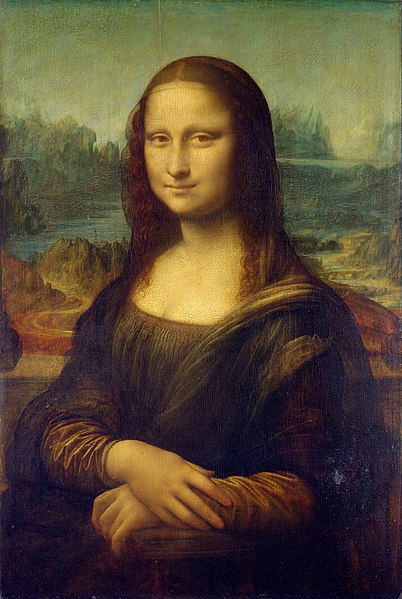
\includegraphics{monalisa}
	\caption[The Mona Lisa]{The Mona Lisa.\\ 
	\url{https://commons.wikimedia.org/wiki/File:Mona_Lisa,_by_Leonardo_da_Vinci,_from_C2RMF_retouched.jpg}}
	\labfig{marginmonalisa}
\end{marginfigure}
 % Deep Blue Brute Force, Machine Translation, Economic Models. 

\pagelayout{wide} % No margins
\addpart{Deep Learning Concepts: layered statistical representations} % It's all just numbers, yo!
\pagelayout{margin} % Restore margins

\setchapterpreamble[u]{\margintoc}
\chapter{How Models Read Data}
\labch{intro}

\section{Numerical Data}

This is some text and a link to 
Hey if you want to site something on the side use\sidecite{Andreu2021}


\section{Words}
\section{Sounds}
\section{Images}
\section{Video}
\section{Mixed Datasets}


\begin{lstlisting}[style=kaolstplain,linewidth=1.5\textwidth]
cd myproject
docker run tensorflow
#profit!
\end{lstlisting}

\url{tex.stackexchange.org} for help.
 

\setchapterpreamble[u]{\margintoc}
\chapter{Machine Learning Methods}
\labch{intro}


are you predicting the right thing? Are you really predicting how valuable the company is or just whether it'll be the next meme stock?

“I hope for some sort of peace—but I fear that machines are ahead of morals by some centuries and when morals catch up there'll be no reason for any of it.” Harry Truman, 1945 \sidecite{McCullough1992}

Representation, "fixing the training set" \sidecite{Christian2020}, or the Impossibility of Fairness from a model.

TODO talk about these books
\cite{Oneil2017}
\cite{Perez2019}
\cite{Blackman2022Jul}
\cite{Christian2020}



"AI Scientists disagree as to whether these language networks posess true knowledge or are just mimicking humans by remembering the statistics of millions of words. I don't beloive any kind of deep learning network will achieve the goal of AGI if the network doesn't model the world the way the brain does. Deep learning networks work well, but not because they solved the knowledge representation problem. They work well because they avoided it completely, relying on statistics and lots of data instead. How deep learning networks work is clever, their performance impressive, and they are commercially valuable. I am only pointing out that they don't possess knowledge and, therefore, are not on the path to having the ability of a five-year-old child." \cite{hawkins_2022}


"The second requirement of goal-misalignment risk is that an intelligent machine can commandeer the Earth's resources to pursue its goals, or in other ways prevent us from stopping it... We have similar concerns with humans. This is why no singer person or entity can control the entire internet and why we require multiple people to launch a nuclear missile. Intelligent machines will not develop misaligned goals unless we go to great lengths to endow them with that ability. Even if they did, no machine can commandeer the world's resources unless we let it. We don't let a single human, or even a small number of humans, control the world's resources. We need to be similarly careful with machines." \cite{hawkins_2022}

\begin{lstlisting}[style=kaolstplain,linewidth=1.5\textwidth]
cd myproject
docker run tensorflow
#profit!
\end{lstlisting}

\url{tex.stackexchange.org} for help.

 

\pagelayout{wide} % No margins
\addpart{The Chaotic Black Box: statistical inference with a billion or so parameters} 
\pagelayout{margin} % Restore margins

\setchapterpreamble[u]{\margintoc}
\chapter{Classifiers}
\labch{intro}


Online Advertising, Justice, Job Applications, Creditworthiness, Getting Insurance (Weapons of Math Destruction), Civic Life, /sidecite{Oneil2017} ; The Default Male, Invisible Women effects snow clearing schedules and drug discovery 

\begin{lstlisting}[style=kaolstplain,linewidth=1.5\textwidth]
cd myproject
docker run tensorflow
#profit!
\end{lstlisting}

\url{tex.stackexchange.org} for help.
 

\setchapterpreamble[u]{\margintoc}
\chapter{Transformers}
\labch{intro}

\section{Style Transfer}
\section{Translation}
\section{Text Generation}

GPT-3, BERT and Bloom

\section{Image Generation and Stable Diffusion}

Link some cool shit here, Draw Owl!

\section{The Ethics of Transforming}

 

\setchapterpreamble[u]{\margintoc}
\chapter{Ensembles and Mathematical Chaos}
\labch{intro}

\section{Interacting Layers of Statistical Understanding}
\section{Useful Chaos}

 

\appendix % From here onwards, chapters are numbered with letters, as is the appendix convention
\pagelayout{wide} % No margins
\addpart{Appendix}
\pagelayout{margin} % Restore margins

\setchapterstyle{lines}
\setchapterpreamble[u]{\margintoc}
\chapter{????}
\labch{appendix}

Let's say we want to build an ensemble model to analyze poetry, put a haiku into craiyon's online shit, then we categorize the resulting photo. \sidecite{Andreu2021}



 

%----------------------------------------------------------------------------------------

\backmatter % Denotes the end of the main document content
\setchapterstyle{plain} % Output plain chapters from this point onwards

%----------------------------------------------------------------------------------------
%	BIBLIOGRAPHY
%----------------------------------------------------------------------------------------

% The bibliography needs to be compiled with biber using your LaTeX editor, or on the command line with 'biber main' from the template directory

\defbibnote{bibnote}{Here are the references in citation order.\par\bigskip} % Prepend this text to the bibliography
\printbibliography[heading=bibintoc, title=Bibliography, prenote=bibnote] % Add the bibliography heading to the ToC, set the title of the bibliography and output the bibliography note

%----------------------------------------------------------------------------------------
%	NOMENCLATURE
%----------------------------------------------------------------------------------------

% The nomenclature needs to be compiled on the command line with 'makeindex main.nlo -s nomencl.ist -o main.nls' from the template directory

\nomenclature{$c$}{Speed of light in a vacuum inertial frame}
\nomenclature{$h$}{Planck constant}

\renewcommand{\nomname}{Notation} % Rename the default 'Nomenclature'
\renewcommand{\nompreamble}{The next list describes several symbols that will be later used within the body of the document.} % Prepend this text to the nomenclature

\printnomenclature % Output the nomenclature

%----------------------------------------------------------------------------------------
%	GLOSSARY
%----------------------------------------------------------------------------------------

% The glossary needs to be compiled on the command line with 'makeglossaries main' from the template directory

\setglossarystyle{listgroup} % Set the style of the glossary (see https://en.wikibooks.org/wiki/LaTeX/Glossary for a reference)
\printglossary[title=Special Terms, toctitle=List of Terms] % Output the glossary, 'title' is the chapter heading for the glossary, toctitle is the table of contents heading

%----------------------------------------------------------------------------------------
%	INDEX
%----------------------------------------------------------------------------------------

% The index needs to be compiled on the command line with 'makeindex main' from the template directory

\printindex % Output the index

%----------------------------------------------------------------------------------------
%	BACK COVER
%----------------------------------------------------------------------------------------

% If you have a PDF/image file that you want to use as a back cover, uncomment the following lines

%\clearpage
%\thispagestyle{empty}
%\null%
%\clearpage
%\includepdf{cover-back.pdf}

%----------------------------------------------------------------------------------------

\end{document}
